% vim:ft=tex:ts=2:sw=0
% Author: Plump Albert (plumpalbert@gmail.com)
\documentclass[../nirs.tex]{subfiles}
\usepackage[figuresleft]{rotating}
\usepackage{pdflscape}

\begin{document}
\section{Выявление основных понятий и процессов, их свойств и закономерностей.
Построение ER-диаграммы предметной области}

\subsection{Основные понятия}
Техническое обслуживание (ТО) -- это комплекс организационно-технических
мероприятий и работ, производимых на технике и направленных на поддержание ее в
рабочем состоянии в процессе использования по назначению, с целью повышения
надежности и эффективности работы [\ref{ref:техническое-обслуживание}].

Рабочее состояние -- состояние транспортного средства, при котором оно способно
выполнять заданные функции с параметрами, установленными в
нормативно-технической документации [\ref{ref:рабочее-состояние}].

Текущий ремонт (ТР) -- устранение мелких неисправностей и отказов автомобиля.
Способствует выполнению установленных норм пробега автомобиля до капитального
ремонта. Текущий ремонт заключается в проведении разборочно-сборочных,
слесарных, сварочных и других работ, а также в замене деталей в автомобиле
(прицепе, полуприцепе) [\ref{ref:му-ремонт-и-техническое-обслуживание}].

Календарное планирование -- распределение во времени видов деятельности.
Календарное планирование представляет собой составление на основе календаря
таблицы, в которой по датам расписаны мероприятия, которые нужно провести, либо
принять в них участие. Планирование бывает персональным или групповым. В
групповом планировании определяемые мероприятия и действия должны быть
согласованы группой участников. Составляемые планы могут быть закрытыми для
посторонних лиц, либо открытыми, где они играют роль объявлений
[\ref{ref:календарное-планирование}].

\subsection{Основные процессы}
Разрабатываемая информационная система должна обеспечивать выполнение следующих
бизнес-процессов:
\begin{itemize}

  \item обеспечивать просмотр информации о конкретном автомобиле;

  \item обеспечивать просмотр и редактирование информации о текущем статусе
  работ;

  \item обеспечивать просмотр и редактирование информации о сотрудниках;

  \item обеспечивать просмотр информации об израсходованных ресурсах;

  \item отображать график прохождения технического обслуживания техники.

\end{itemize}

\subsection{Построение ER-диаграммы предметной области}

При проектировании структуры предметной области были определены сущности
(объекты, явления), отражающие ее, а также информационные потребности
пользователей системы.

Классовая диаграмма системы представлена на рисунке \ref{fig:2_1_er_diagram}.

\clearpage
\begin{landscape}

\begin{figure}[hp!]
  \centering
  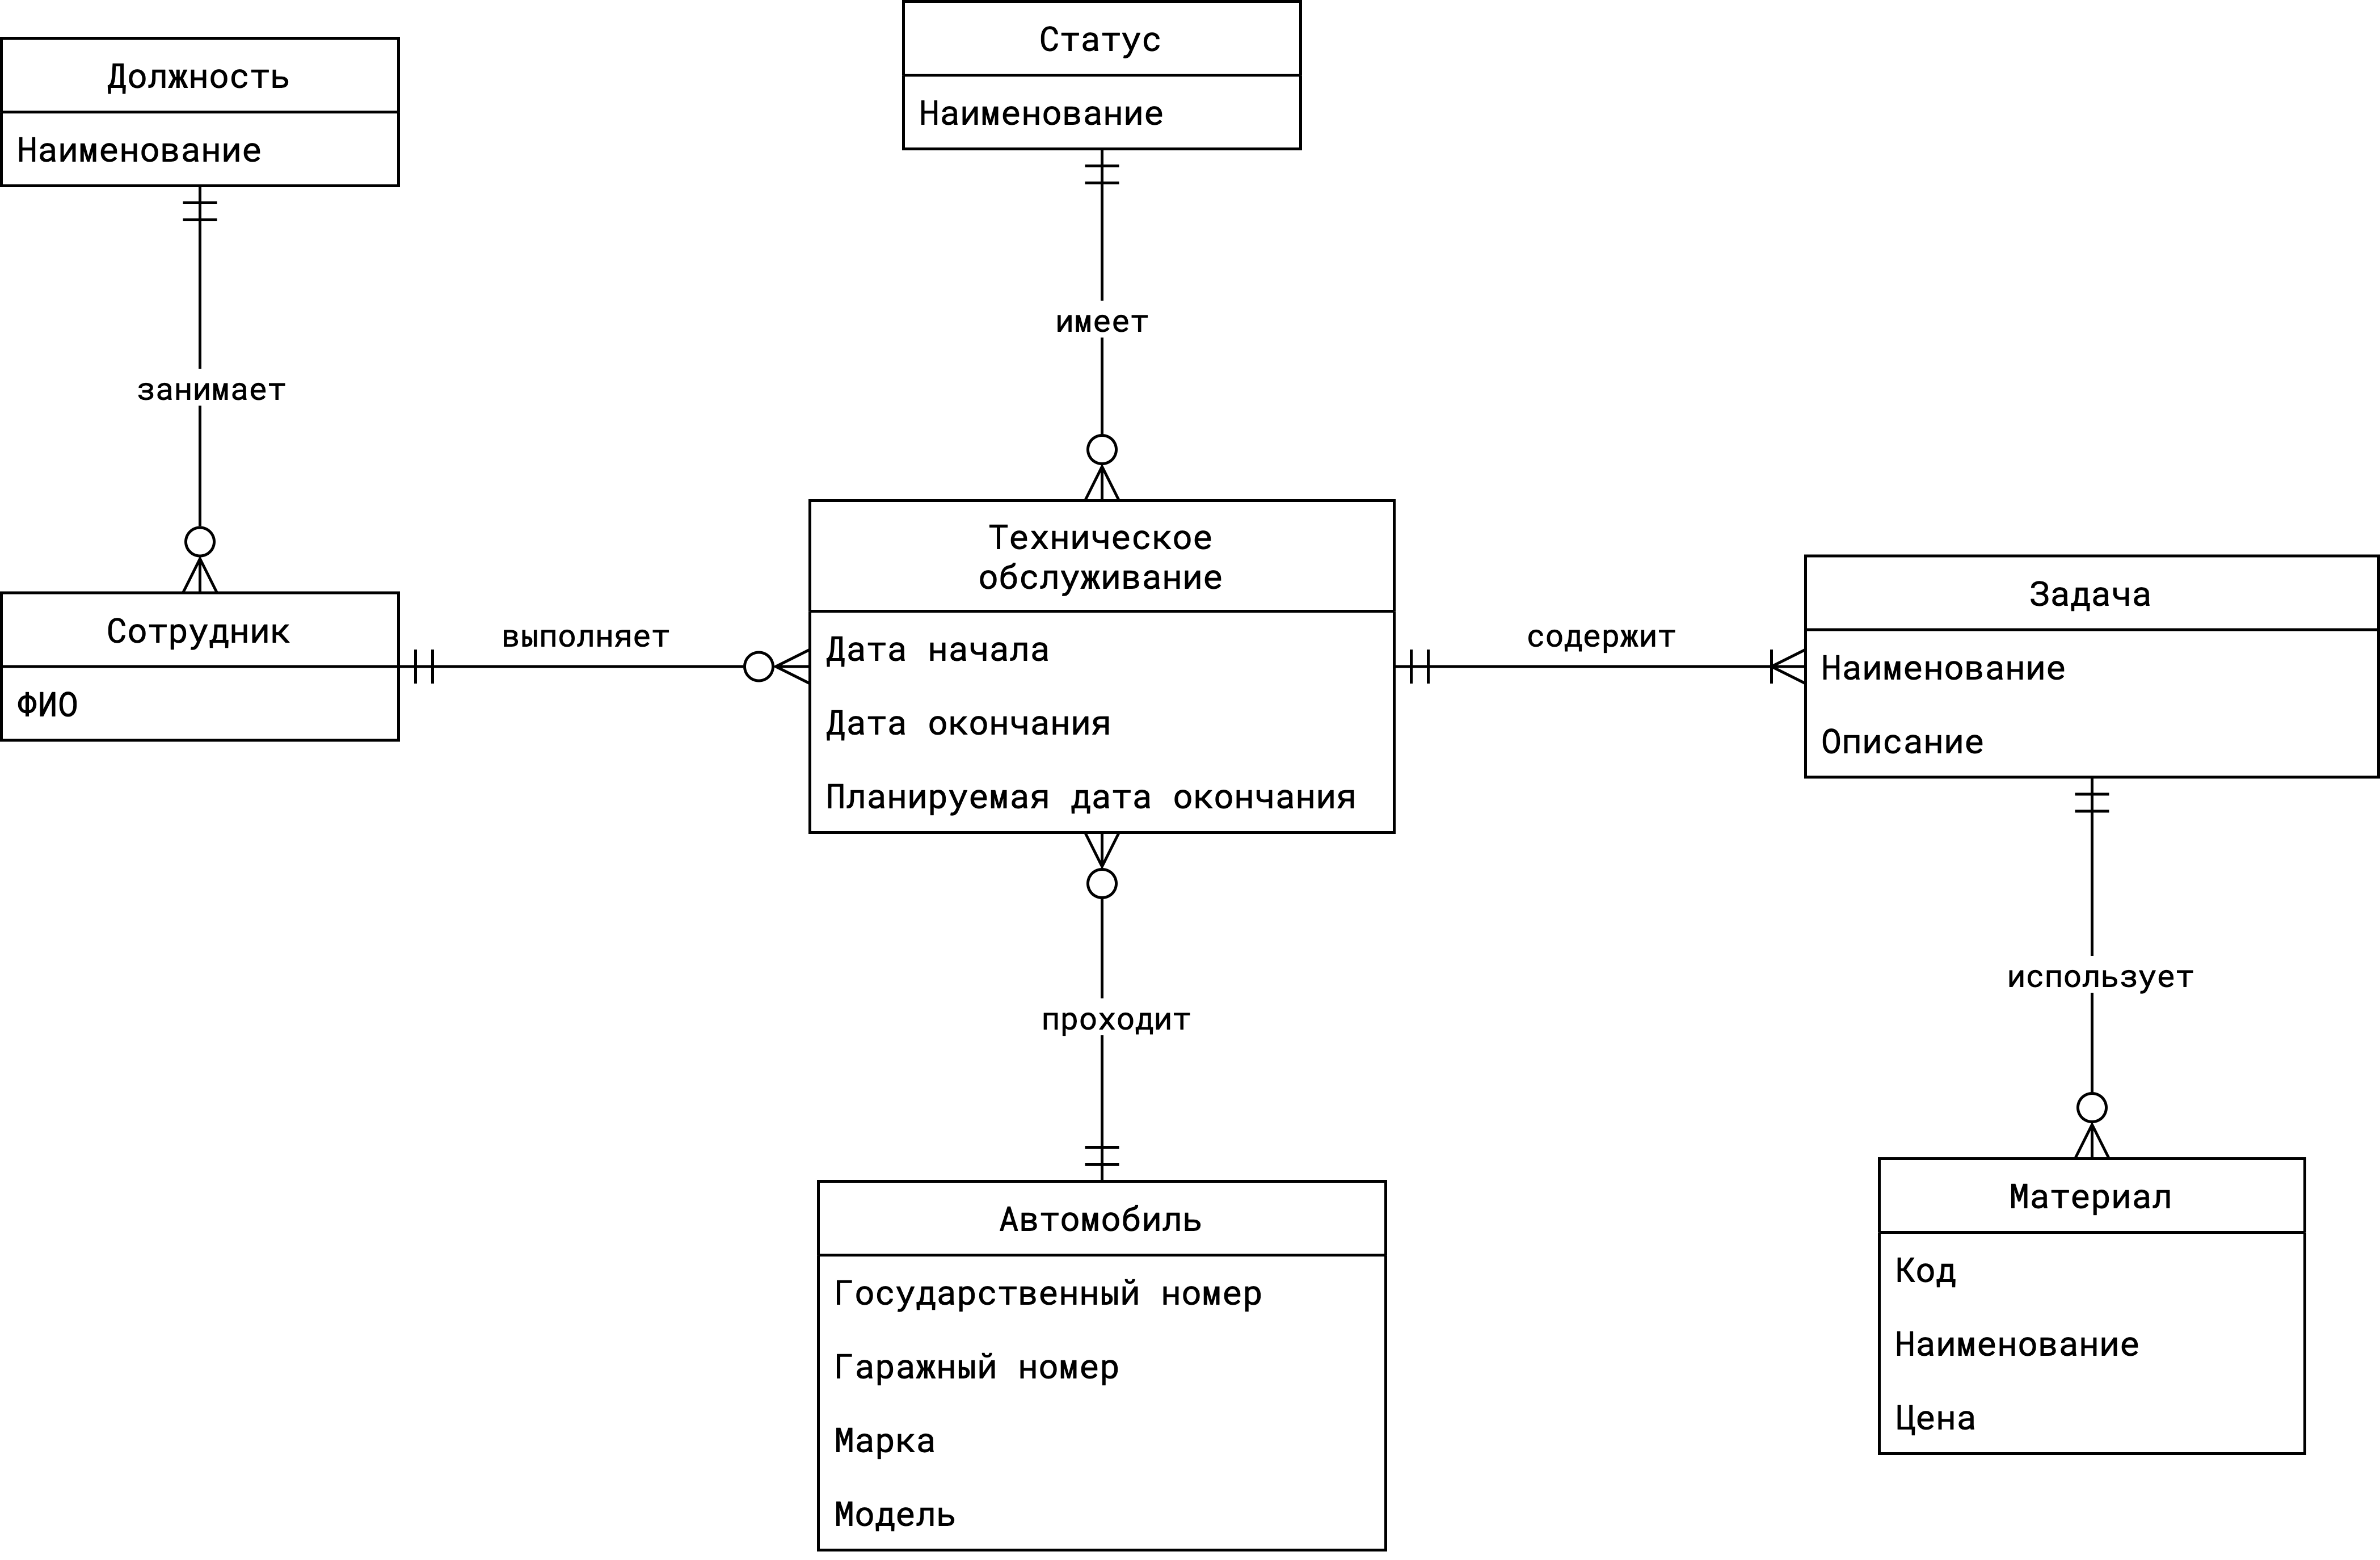
\includegraphics[keepaspectratio,
                   width=1.4\textwidth]{./images/er-2.png}
  \caption{ER-диаграмма системы}
  \label{fig:2_1_er_diagram}
\end{figure}

\end{landscape}
\clearpage

Сущность \textquote{Автомобиль} содержит информацию о конкретной единице
техники, такую как государственный регистрационный номер, гаражный номер, марка
и модель автомобиля.

Сущность \textquote{Сотрудник} представляет собой пользователя системы.
В ней содержится имя сотрудника. Каждому сотруднику соответствует должность,
описанная сущностью \textquote{Должность}.

Сущность \textquote{Техническое обслуживание} содержит информацию о датах начала
и окончания работ, а также планируемый срок выполнения обслуживания. Каждое
обслуживание включает в себя перечень работ, описанных сущностью
\textquote{Задача}. В ней хранится информация о виде работы, которую необходимо
выполнить, а также пояснение к ней.

При выполнении задач расходуются материалы, описанные сущностью
\textquote{Материал}. В ней хранится информация наименование материала, его
идентификационный код и цена.

\end{document}
